\section{Matematyczny model emocji}\label{rozdzial_modelEmocji}
W~celu realizacji postawionego zadania należy zdefiniować emocje matematycznie. Jednym z~podejść stosowanych w~pracach o~podobnej tematyce jest wykorzystanie etykiet mówiących o emocjach. Każdy z~utworów etykietowano z~wykorzystaniem przymiotników takich jak np. ,,smutny'', ,,wesoły'', ,,relaksujący''.  Innym rozwiązaniem jest określanie emocji z~wykorzystaniem dwuwymiarowej przestrzeni opracowanej przez Russell'a\cite{emotion} i~podobnie postąpiono w~niniejszej pracy. W~tym przypadku, emocje określona są przy pomocy dwóch parametrów: pobudzenia(ang. \emph{arousal}) oraz zadowolenia(ang. \emph{valence}), co przedstawia rysunek \ref{russelModel}. Model ten zakłada, że wszystkie emocje wynikają z~dwóch niezależnych systemów neurofizjologicznych\footnote{system neurofizjologiczny - system układu nerwowego} w~kontekście do poprzednich teorii zakładających istnienie niezależnych systemów dla każdej podstawowej emocji. Wyniki najnowszych badań są jednak bardziej konsystentne z~nowszym podejściem\cite{emotion}.

% https://www.researchgate.net/publication/258273035_The_physiological_Measurements_as_a_Critical_Indicator_in_Users'_Experience_Evaluation

\begin{figure}[ht!]
\centering
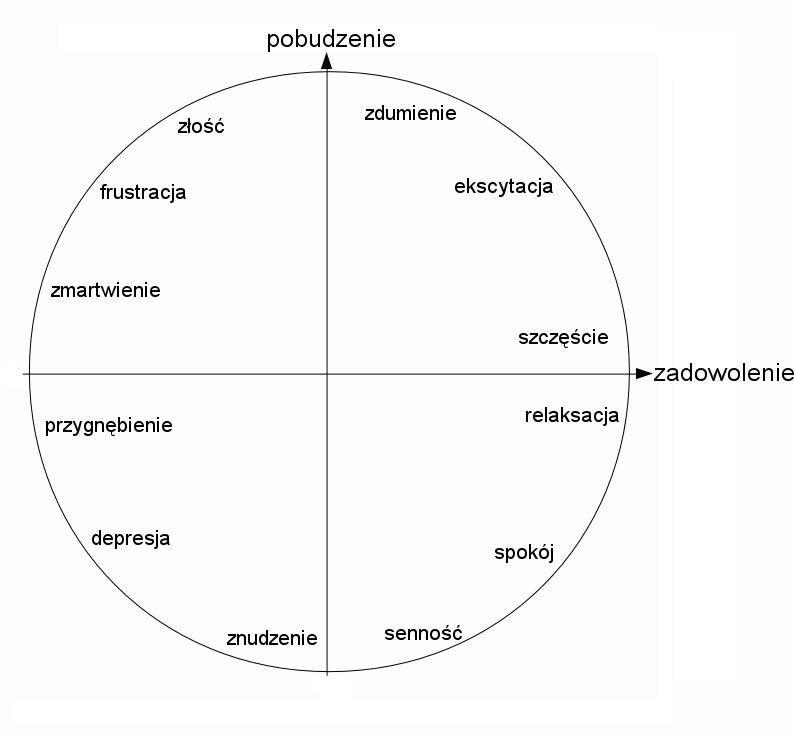
\includegraphics[scale=0.5]{res/emotionModel.png}
\caption{Model emocji według Russela}\label{russelModel}
\end{figure}